\marginpar{\href{https://youtu.be/6oV3pKLgW2I}{Video}}

\begin{figure}[ht]
\centering
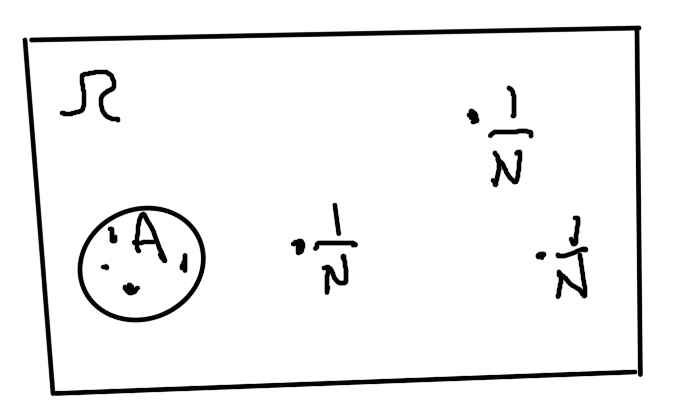
\includegraphics[width=5cm, height=4cm]{images/L04/counting.jpeg}
\caption{Counting}
\end{figure}

$\Omega=|N|$ - Need to determine N.
$|A|=n$

$$
P(A)=n\cdot \frac{1}{N}
$$

\marginpar{(3:30)} The most common trick is when considering a set, describe the outcomes through a sequential process.

\begin{figure}[ht]
\centering
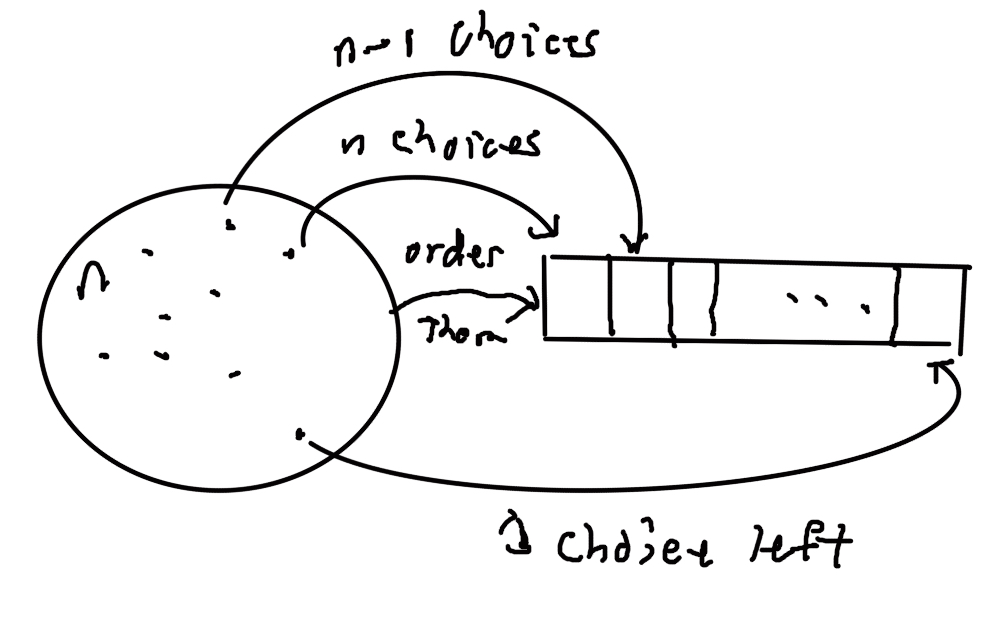
\includegraphics[width=5cm, height=4cm]{images/L04/seq_counting.jpeg}
\caption{Sequential Counting}
\end{figure}


Number of subsets of $\{1,,2, \ldots, n\}$.  For each element we have 2 choices: include/exclude.

\begin{align*}
    \underbrace{2\cdot 2\cdots 2}_{n} = 2^n
\end{align*}

\subsection{Example: Probability 6 rolls of 6-sided die are all different numbers}

\marginpar{(11:05)}

One outcome: $P(2,3,3,1,6,5)=P(2)P(3)P(3)P(1)P(6)P(5)=(\frac{1}{6})^6$

Number of elements in sample space: $\Omega=6^6$

\begin{align*}
\frac{|A|}{|\Omega|} = \frac{6!}{6^6}
\end{align*}

\marginpar{(16:30)}

Interested in subsets that have exactly k elements.

\begin{figure}[ht]
\centering
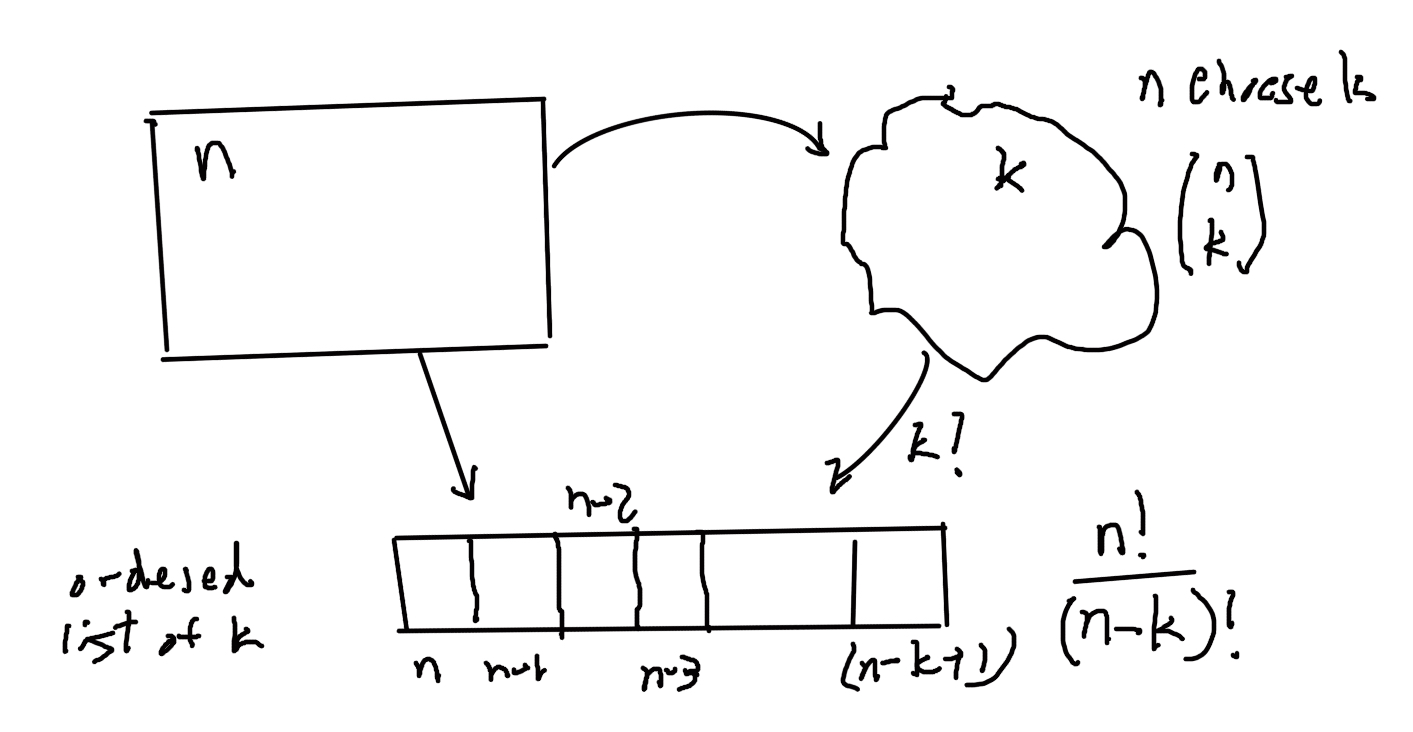
\includegraphics[width=5cm, height=4cm]{images/L04/sel_k_elems.jpeg}
\caption{Select k elements}
\end{figure}

e.g. N people in group and want to form k committees.

\begin{align*}
n(n-1)(n-2)\cdots (n-k+1)=\frac{n!}{(n-k)!} \quad choices
\end{align*}

\marginpar{(22:30)}

Hence:
\begin{align*}
\binom{n}{k}\cdot k! = \frac{n!}{(n-k)!} \Rightarrow \binom{n}{k}\frac{n!}{k!(n-k)!}
\end{align*}
This is the binomial coefficient.

\marginpar{(23:45)}

Defn: $0! = 1$

\begin{itemize}
    \item case k=n: $\frac{n!}{n!0!}=1$
    \item case k=0: $\frac{n!}{0!n!}=1$ 
\end{itemize}


\marginpar{(26m)}

$$\sum_{k=0}^n \binom{n}{k} = 2^n$$ \text{ we count the total number subsets}

\subsubsection{Binomial Probabilities}

\marginpar{(28:30)}

\begin{align*}
&P(H)=p\\
&P(HTTHHH)=p(1-p)(1-p)ppp = p^4(1-p)^2\\
&P(HHTTHH)= p^4(1-p)^2, \qquad \text{Same but different order}\\
&p^{\#heads}(1-p)^{\#tails}
\end{align*}

\marginpar{(32:25)}

\# k-head sequence = \# k-element subsets of $\binom{n}{k}$

\begin{figure}[h]
\centering
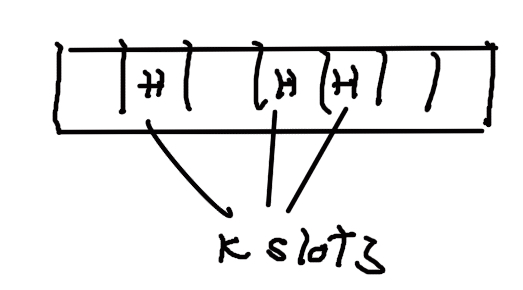
\includegraphics[width=5cm, height=4cm]{images/L04/k_slots.jpeg}
\caption{k slots}
\end{figure}

\begin{align}
\sum_{k=0}^{n} \binom{n}{k} p^k(1-p)^{n-k}=1  
\label{eq:binomial_pmf}
\end{align}

\myequations{Binomial PMF}

$k=0,1,\ldots,n$ are binomial probabilities

\subsubsection{Coin Toss Experiment}

\begin{figure}[h]
\centering
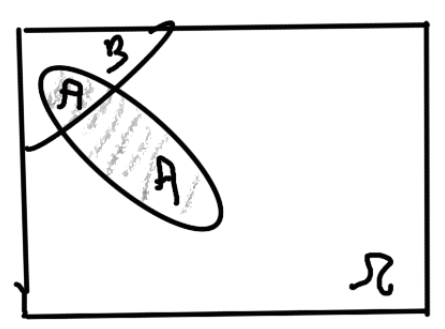
\includegraphics[width=5cm, height=4cm]{images/L04/coin_toss_exp.jpeg}
\caption{Coin Toss Experiment}
\end{figure}

Event B = \{3 out of 10 heads\}, Event A=\{first two tosses H\}

Events of $\Omega$ are not equally likely.

B: $\binom{10}{3}$, A: only third is uncertain: 8

\subsection{Partitions}

\marginpar{(42:55)}

\begin{figure}[h]
\centering
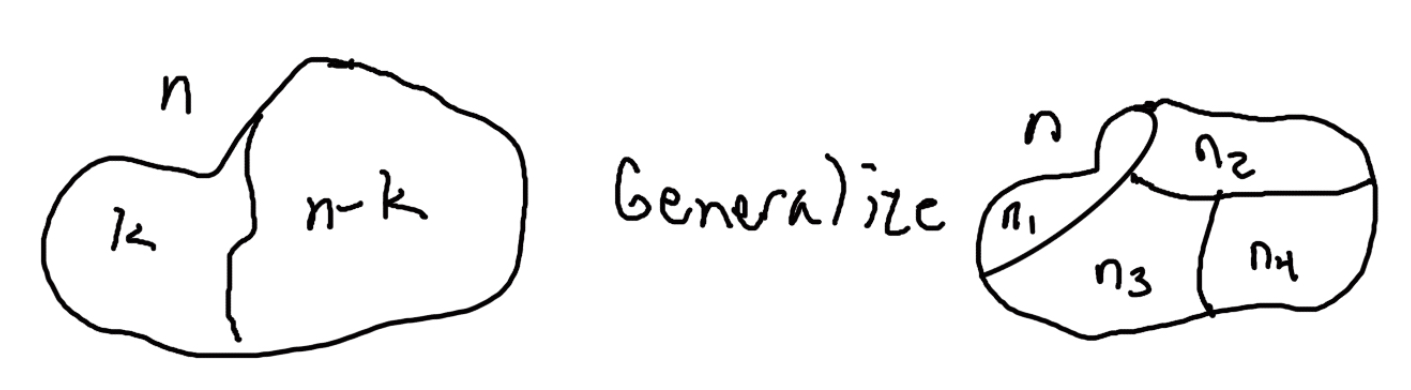
\includegraphics[width=8cm, height=4cm]{images/L04/generalize.jpeg}
\caption{Generalize}
\end{figure}

\begin{align*}
\binom{52}{13}\binom{39}{13}\binom{26}{13}\binom{13}{13}\\
    % {52 \choose 13}{39 \choose 13}{26 \choose 13}{13 \choose 13}
\end{align*}

\begin{align*}
    \frac{52!}{13!39!} \cdots = \frac{52!}{13!13!13!13!}
\end{align*}

\begin{align}
    \frac{n!}{n_1!n_2!n_3!n_4!}
\end{align}

$P(\text{each player gets ace}) = $ (see text book)

\subsection{Stars and Bars}
